\providecommand{\main}{../../../..}
\documentclass[\main/dresen_thesis.tex]{subfiles}
\begin{document}
  \label{sec:colloidalCrystals:nanoparticle:sas}

  \begin{figure}[htbp]
    \centering
    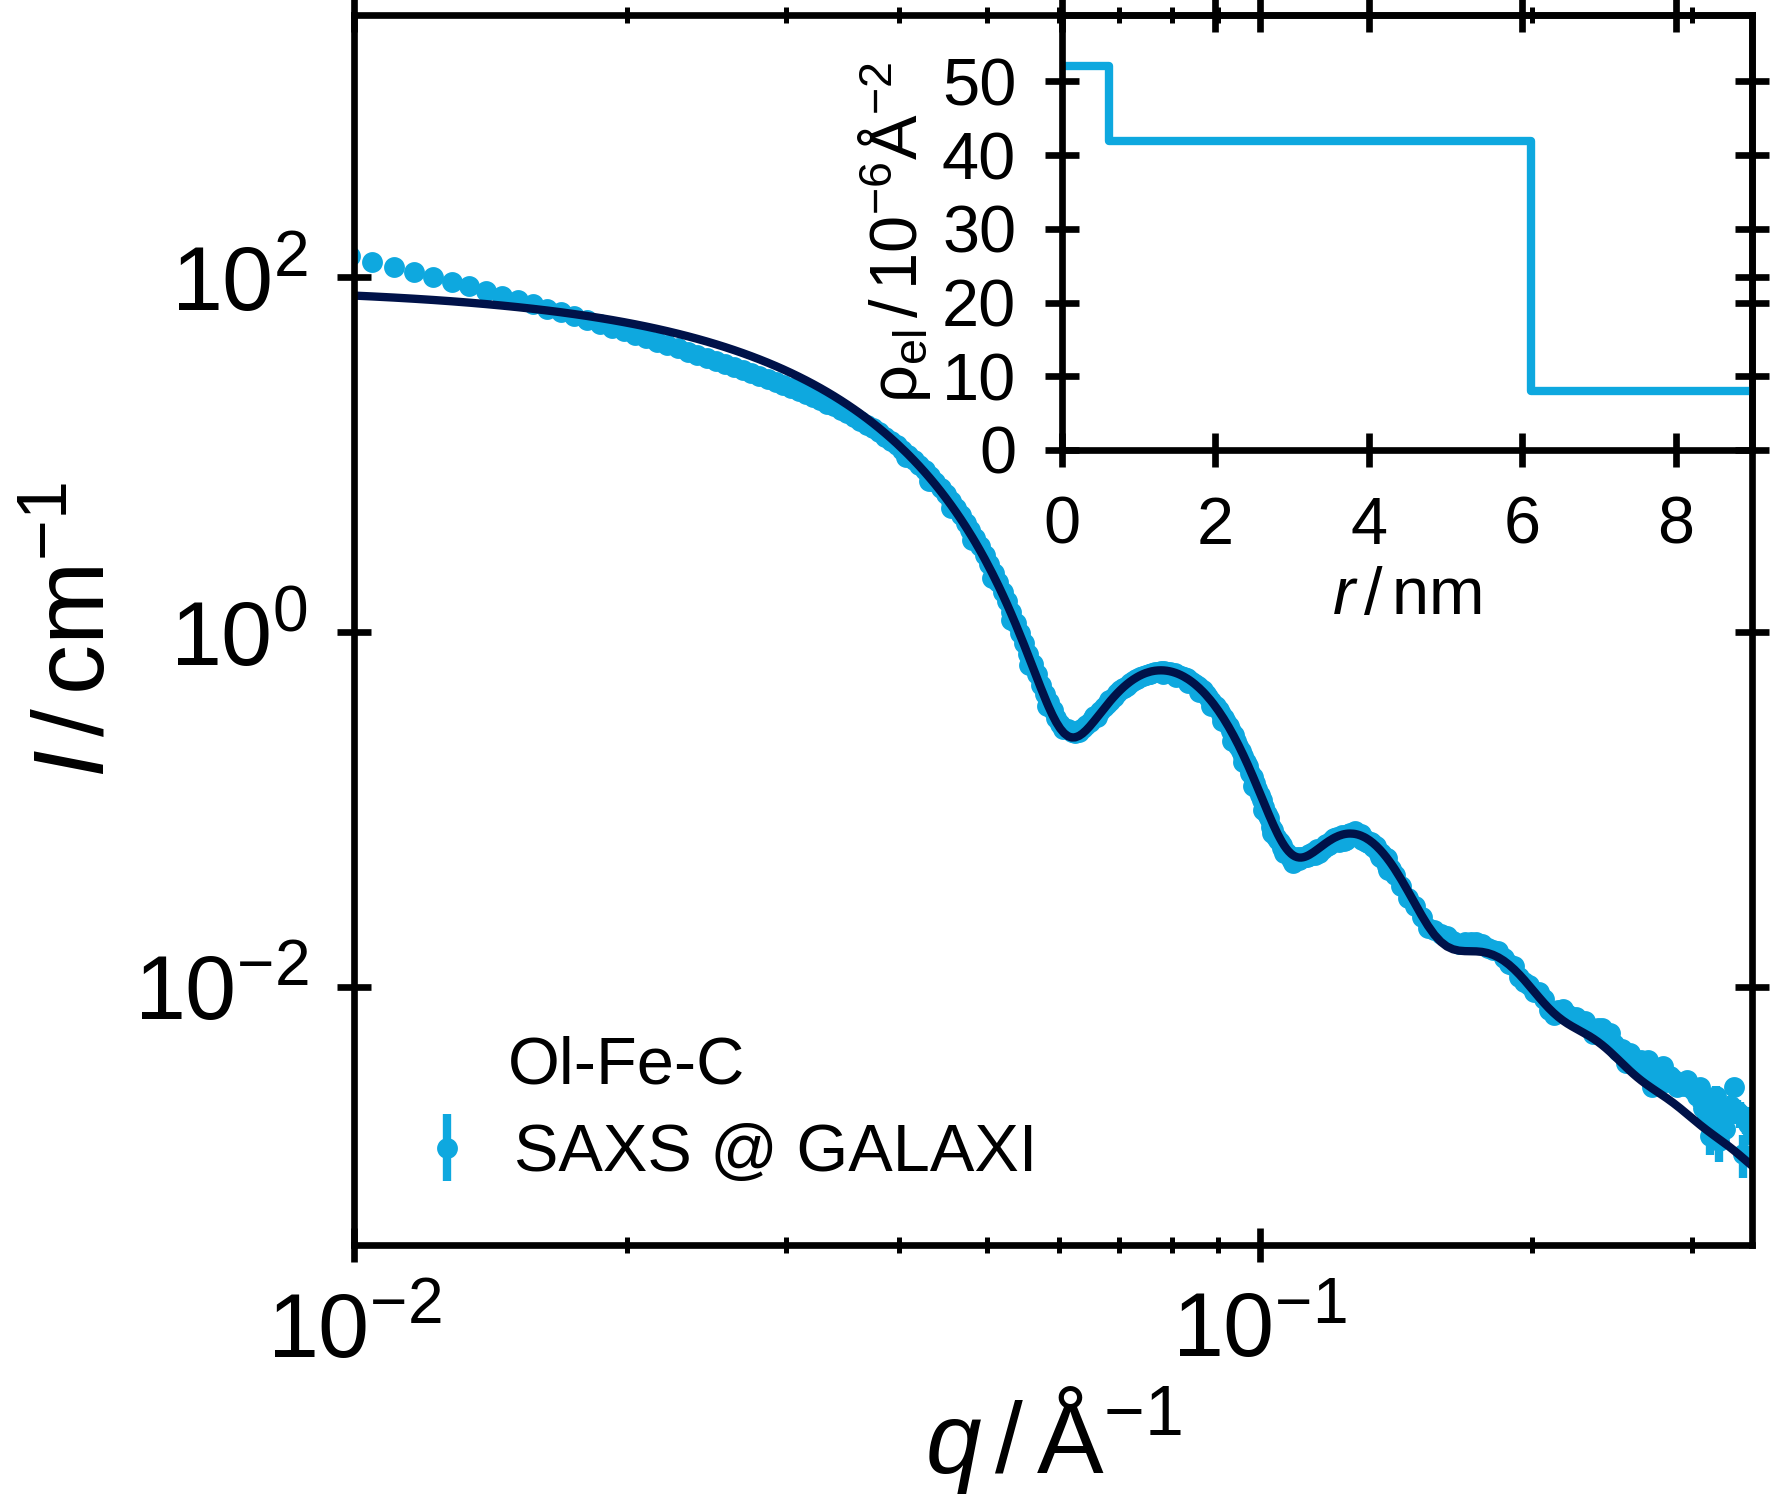
\includegraphics{colloidalCrystals_SAS_Ol-Fe-C_SAXS}
    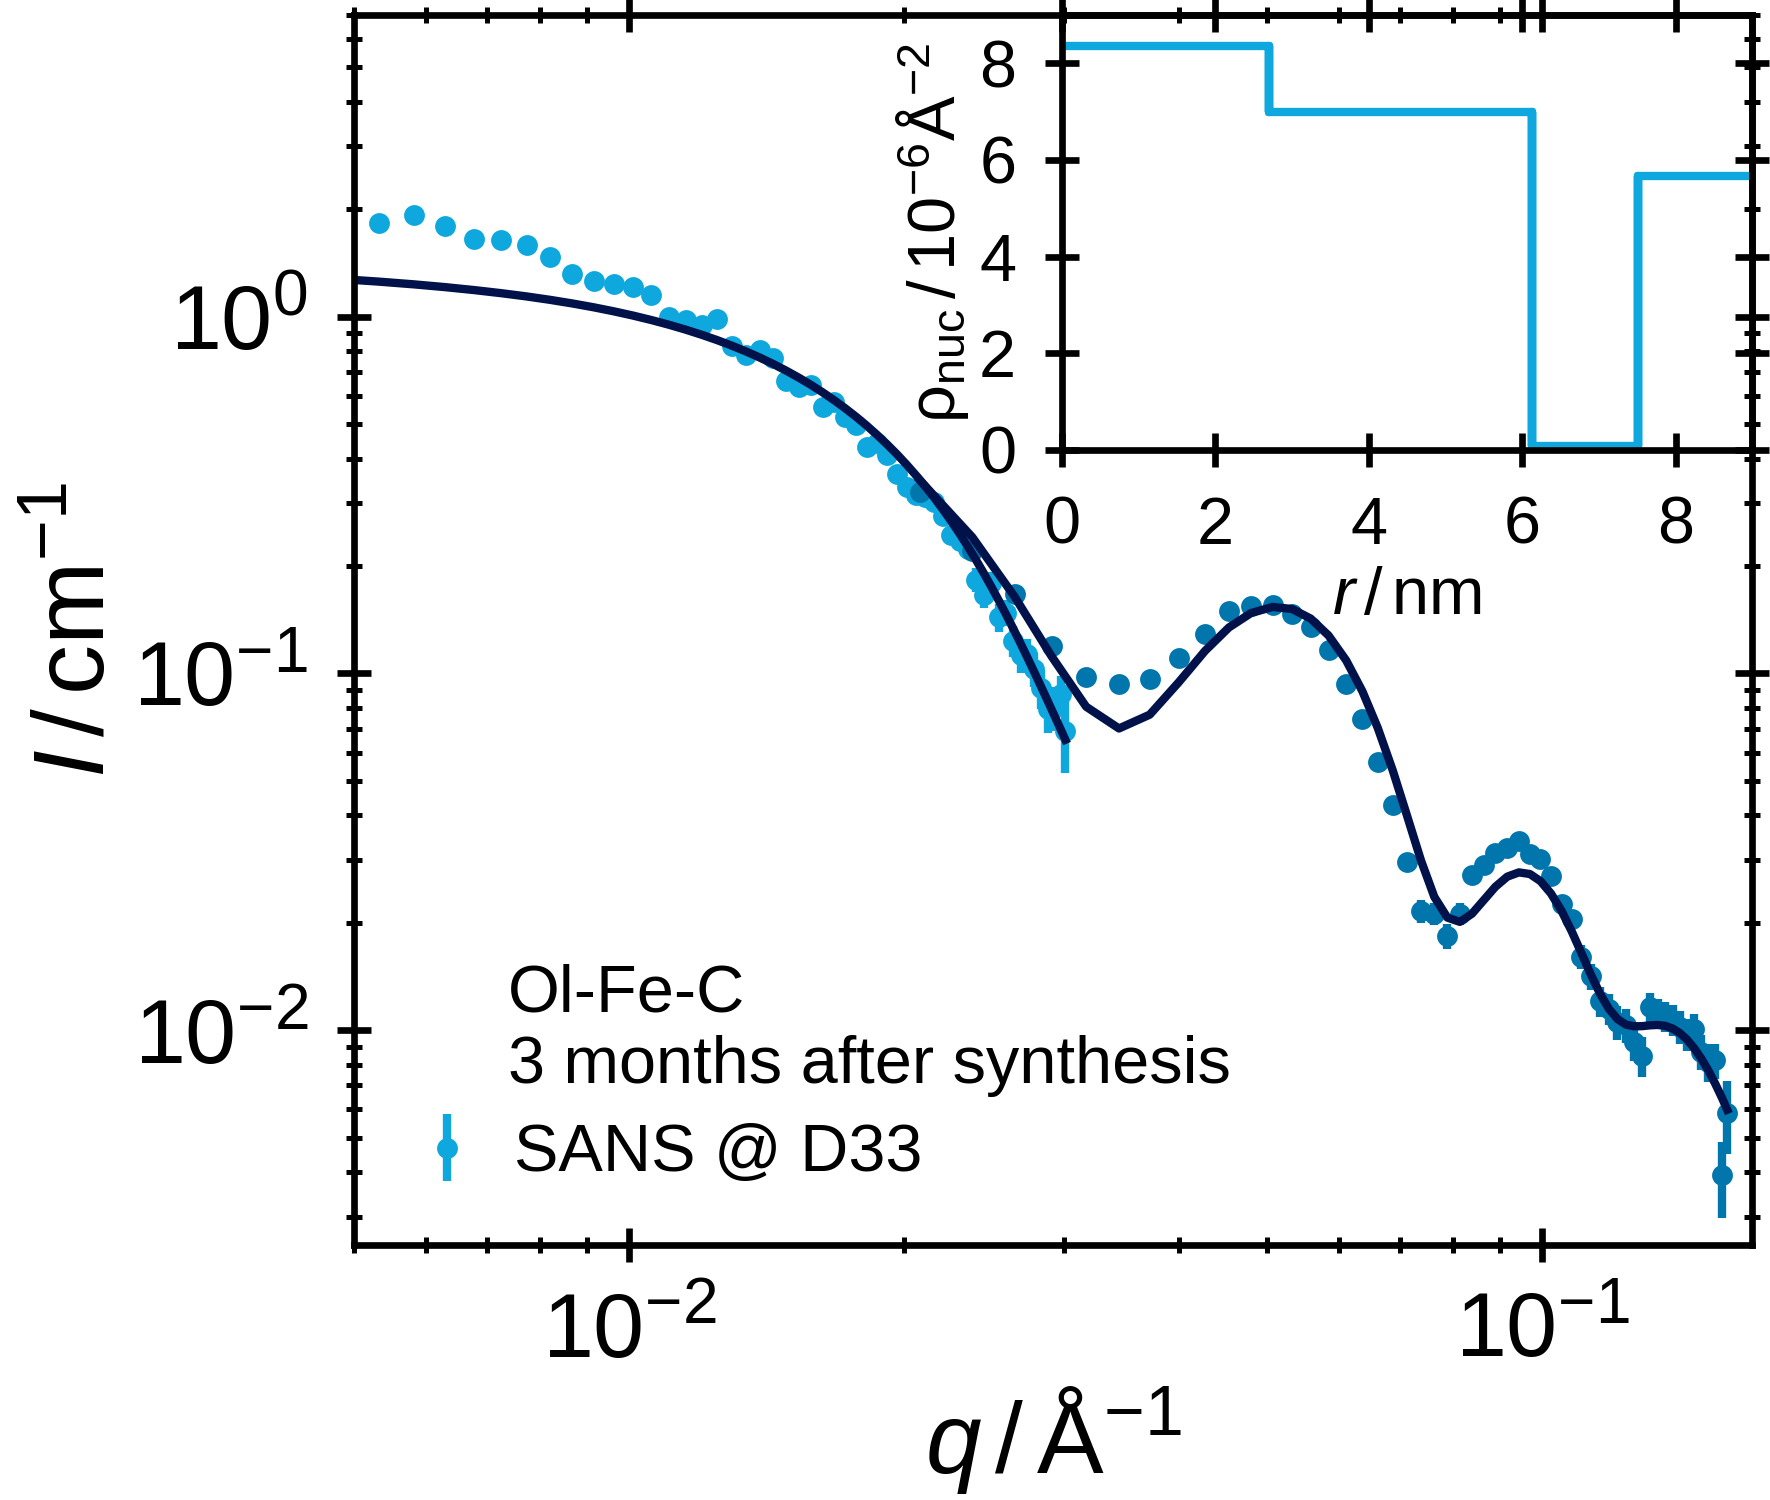
\includegraphics{colloidalCrystals_SAS_Ol-Fe-C_SANS}
    \caption{\label{fig:colloidalCrystals:nanoparticle:sas}Azimuthally averaged small-angle X-ray (left) and neutron (right) scattering of Ol-Fe-C. SAXS is fit a to homogeneous superball with the determined shape shown as inset, whereas SANS to a core-shell superball form factor with an additional surfactant shell, where the profile along a principal axes is shown in the inset.}
  \end{figure}
  The nanocubes Ol-Fe-C are characterized by both small-angle X-ray and neutron scattering with the intent to precisely determine the particle size, size distribution, core-shell morphology and particle magnetization.
  The SAXS data that was measured at the GALAXI instrument (\refsec{ch:lss:galaxi}) and the SANS data measured at D33 (\refsec{ch:lss:d33}) are shown after data reduction in \reffig{fig:colloidalCrystals:nanoparticle:sas}.
  Both SAXS and SANS show visible minima in the form factor up to the third order.
  It is furthermore well visible in both data sets that the form factor does not form a plateau at low $q$ values, but increases still.
  This is a sign that interparticle interactions are additionally present in the data and that possibly a too high particle concentration was chosen for the measurements.
  The low-$q$ power law is determined by a fit in SAXS to $-1.47(1)$, which is in-between the power law of $-1$ expected for rods and $-2$ for disks \cite{Guinier_1955_Smalla}.

  Both data sets are fitted to the form factor of superball form factor with a core-shell structure and an additional oleic acid surfactant shell.
  The SAXS data is considered as dispersed in toluene, whereas the SANS data has a toluene-\textit{d8} matrix.
  The scattering length density of the core and shell are fixed to w\"ustite and magnetite as this is expected from literature \cite{Wetterskog_2013_Anoma} and was estimated in the previous characterization by XRD in \refsec{sec:colloidalCrystals:nanoparticle:xrd}.
  The best fits are respectively shown in \reffig{fig:colloidalCrystals:nanoparticle:sas}.
  The estimated cube morphology and it's rounded edges are depicted in the inset of the SAXS data.
  The parameters of the two form factors are given in \reftab{tab:colloidalCrystals:nanoparticle:sas}.

  Both data sets are described by a superball with a radius of $6.13(2) \unit{nm}$ and a superball exponent of $2.15(7)$.
  The superball radius corresponds to a superball edge length of $12.26(4) \unit{nm}$.
  For SAXS a homogeneous superball is obtained as best fit, whereas for SANS a core-shell structure with a magnetite shell thickness of $3.4(2) \unit{nm}$ is refined.
  It is noteworthy that the SANS experiment was performed approximately three months after the nanocube synthesis, whereas the SAXS experiment was performed additional five months after the SANS experiment.
  The disappearing of the w\"ustite core in SAXS is hence attributed to oxidation of the sample with time.

  Furthermore a size distribution of $7.2(1) \%$ is observed, which is determined by SAXS and confirmed from the SANS fit.
  The value is in excellent agreement with the size distribution of $7.3(5) \%$ that was observed by manually counting particles in TEM.
  % The instrumental resolution parameters in SANS are fit to $\Delta \theta_\mathrm{11 m} \eq 1.7(1) \unit{mrad}$ and $\Delta \theta_\mathrm{2 m} \eq 2.8(2) \unit{mrad}$.
  % The value at large sample-to-detector distance fits well with the estimated instrumental resolution from the apertures and collimation, sample and detector distances ($1.6 \unit{mrad}$), whereas the parameter at small sample-to-detector distance shows that a better resolution is actually observed than initially estimated ($3.8 \unit{mrad}$).

  \begin{table}[!htbp]
    \centering
    \caption{\label{tab:colloidalCrystals:nanoparticle:sas}Parameters for the spherical core-shell model of Ol-Fe-C.}
    \begin{tabular}{ c | l | l}
      \rule{0pt}{2ex} \textbf{Ol-Fe-C} & \textbf{SAXS} & \textbf{SANS}\\
      \hline
      \rule{0pt}{2ex} $R_\mathrm{core} + D_\mathrm{shell} \, / \unit{nm}$             & \multicolumn{2}{c}{$6.13(2)$} \\
      \rule{0pt}{2ex} $D_\mathrm{shell}\, / \unit{nm}$                                & -            & $3.3(2)$       \\
      \rule{0pt}{2ex} $D_\mathrm{surfactant}\, / \unit{nm}$                           & -            & $1.38(4)$    \\
      \rule{0pt}{2ex} $p $                                                            & \multicolumn{2}{c}{$2.15(7)$} \\
      \rule{0pt}{2ex} $\sigma_{(R+D)}\, / \unit{\%}$                                  & \multicolumn{2}{c}{$7.2(1)$} \\
      \rule{0pt}{2ex} $n \, / \unit{10^{-8} \angstrom^{-3}}$                          & $0.0300(2)$  &  $0.054(1)$ \\
      \hline
      \rule{0pt}{2ex} $\rho_\textsf{w\"ustite} \, / \unit{10^{-6} \angstrom^{-2}}$    & -       & $8.35$\\
      \rule{0pt}{2ex} $\rho_\mathrm{magnetite} \, / \unit{10^{-6} \angstrom^{-2}}$    & $41.85$ & $7.00$\\
      \rule{0pt}{2ex} $\rho_\mathrm{oleic\, acid} \, / \unit{10^{-6} \angstrom^{-2}}$ & -       & $0.078$\\
      \rule{0pt}{2ex} $\rho_\mathrm{solvent} \, / \unit{10^{-6} \angstrom^{-2}}$      & $8.01$  & $5.66$\\
      \hline
      \rule{0pt}{2ex} $\lambda^\mathrm{sans} \, / \unit{\unit{\angstrom}}$            & $1.34$  & $6.00$\\
      \rule{0pt}{2ex} $\Delta \lambda / \lambda \, / \unit{\%}$                       & -       & $4.247$\\
      \rule{0pt}{2ex} $\Delta \theta_\mathrm{11 m} \, / \unit{mrad}$                  & -       & $1.7(1)$\\
      \rule{0pt}{2ex} $\Delta \theta_\mathrm{2 m} \, / \unit{mrad}$                   & -       & $2.8(2)$\\
      \rule{0pt}{2ex} $I_\mathrm{bg} \, / \unit{cm^{-1}}$                             & $0$     & $0$\\
      \hline
      \rule{0pt}{2ex} $c_m \, / \unit{mg\, mL^{-1}}$                                  & $2.4(1)$ & $7.7(1)$\\
      \hline
    \end{tabular}
  \end{table}

  \paragraphNewLine{Magnetic Structure}
    \begin{figure}[tb]
      \centering
      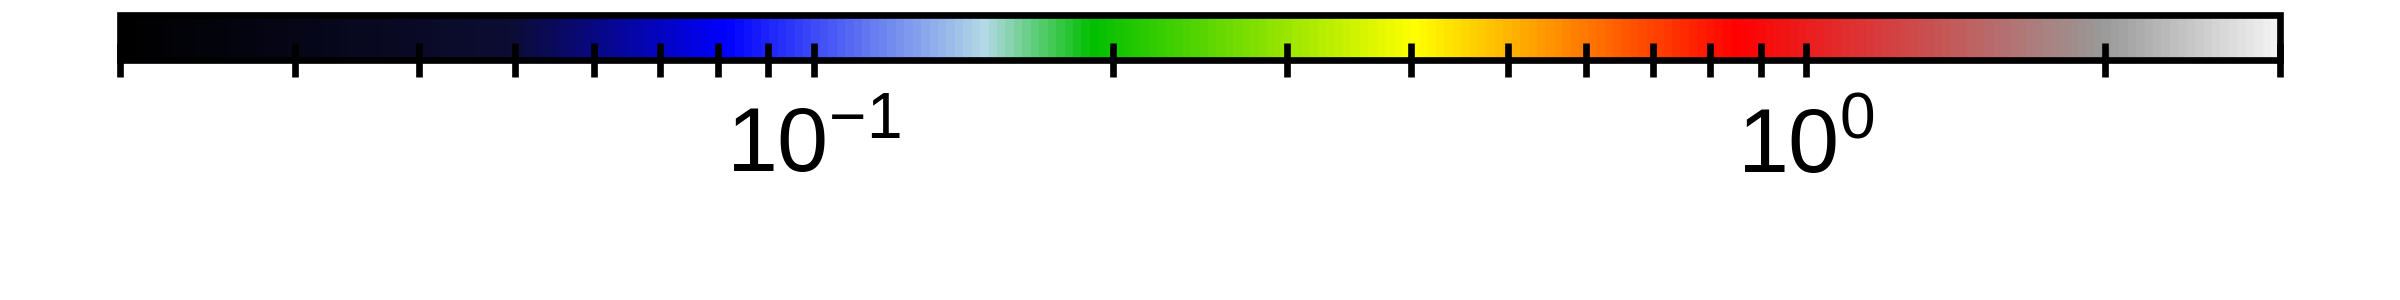
\includegraphics{colloidalCrystals_SANSPOL_SVcbar}
      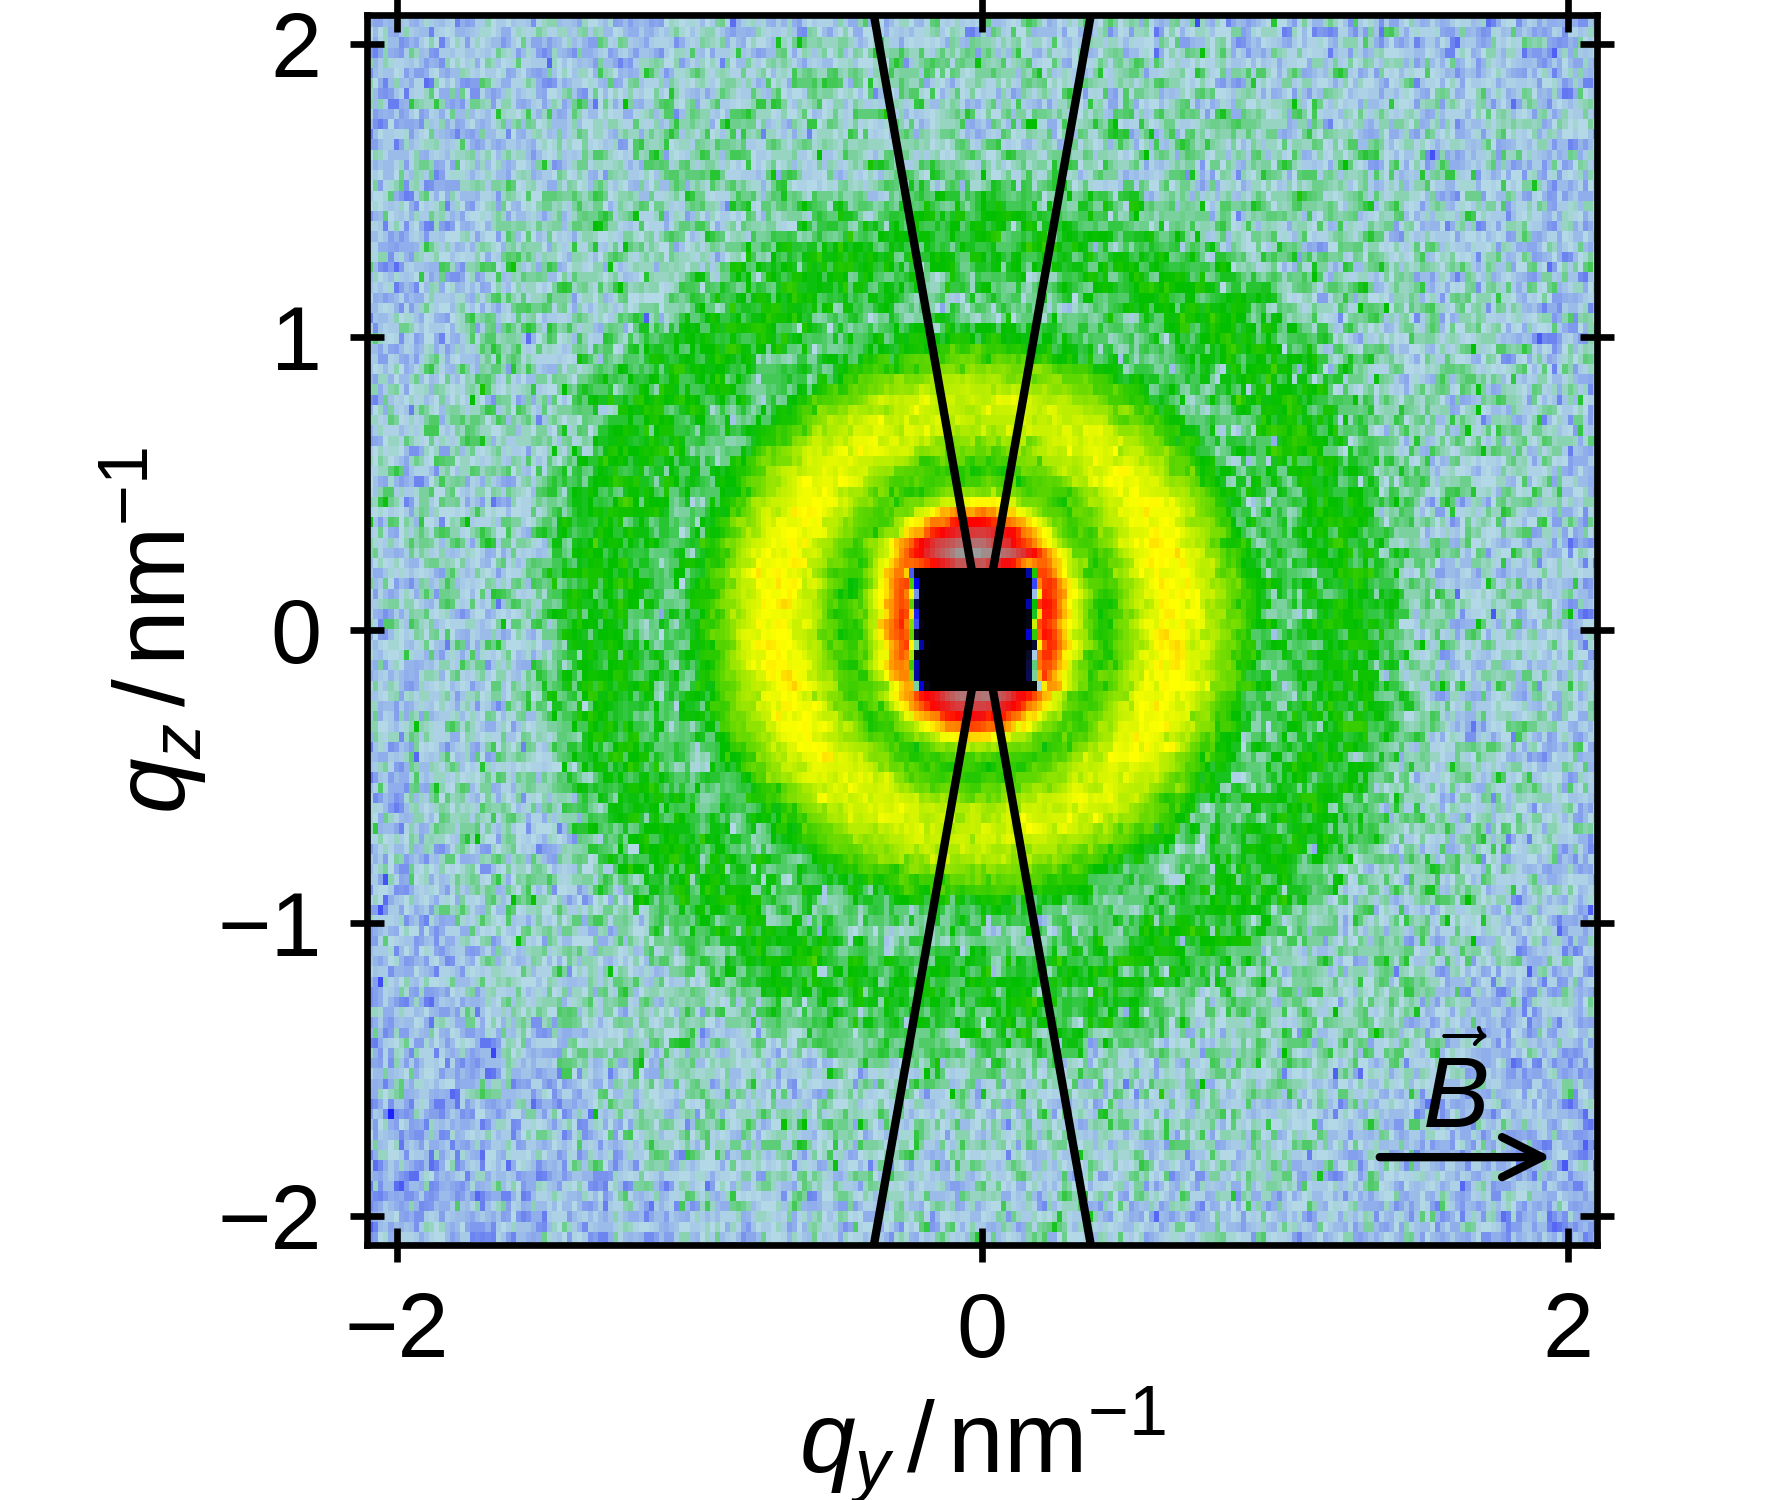
\includegraphics{colloidalCrystals_SANSPOL_MagneticScattering_RFoff}
      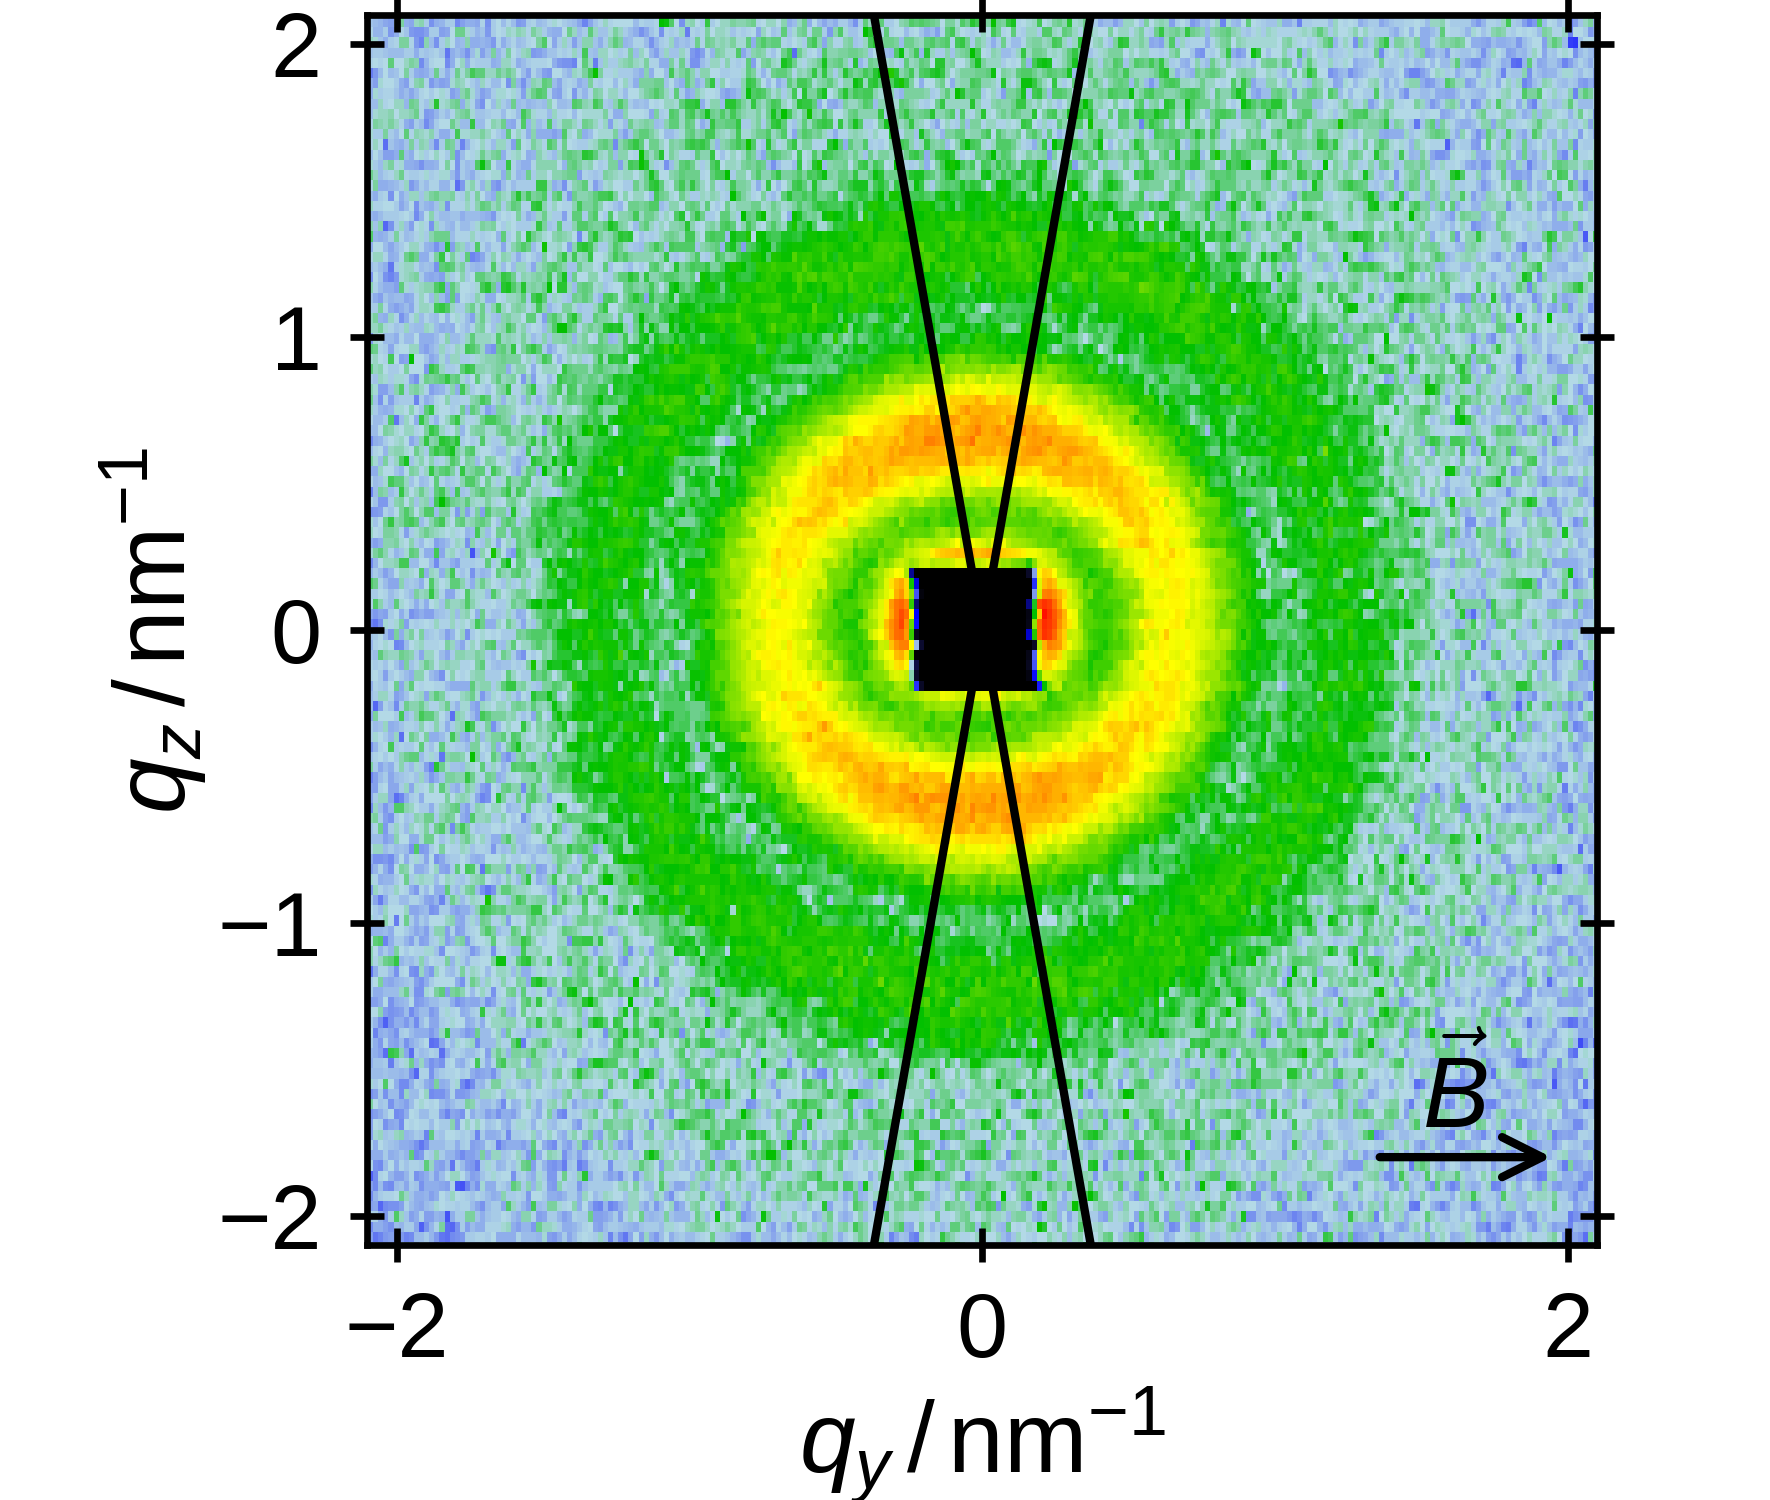
\includegraphics{colloidalCrystals_SANSPOL_MagneticScattering_RFon}
      \caption{\label{fig:colloidalCrystals:nanoparticle:sanspolDetectorImage}$I^{+}$ (left) and $I^{-}$ (right) of the SANSPOL measurements of Ol-Fe-C at the small sample-to-detector distance.}
    \end{figure}

    The nanocubes were furthermore measured with polarized neutrons at D33, while applying a strong magnetic field of $1.234 \unit{T}$.
    The detector data, shown for the short sample-to-detector distance in \reffig{fig:colloidalCrystals:nanoparticle:sanspolDetectorImage}, already shows the strong contrast due to the magnetic scattering contribution along the $q_z$ dimension.

    \begin{figure}[htbp]
      \centering
      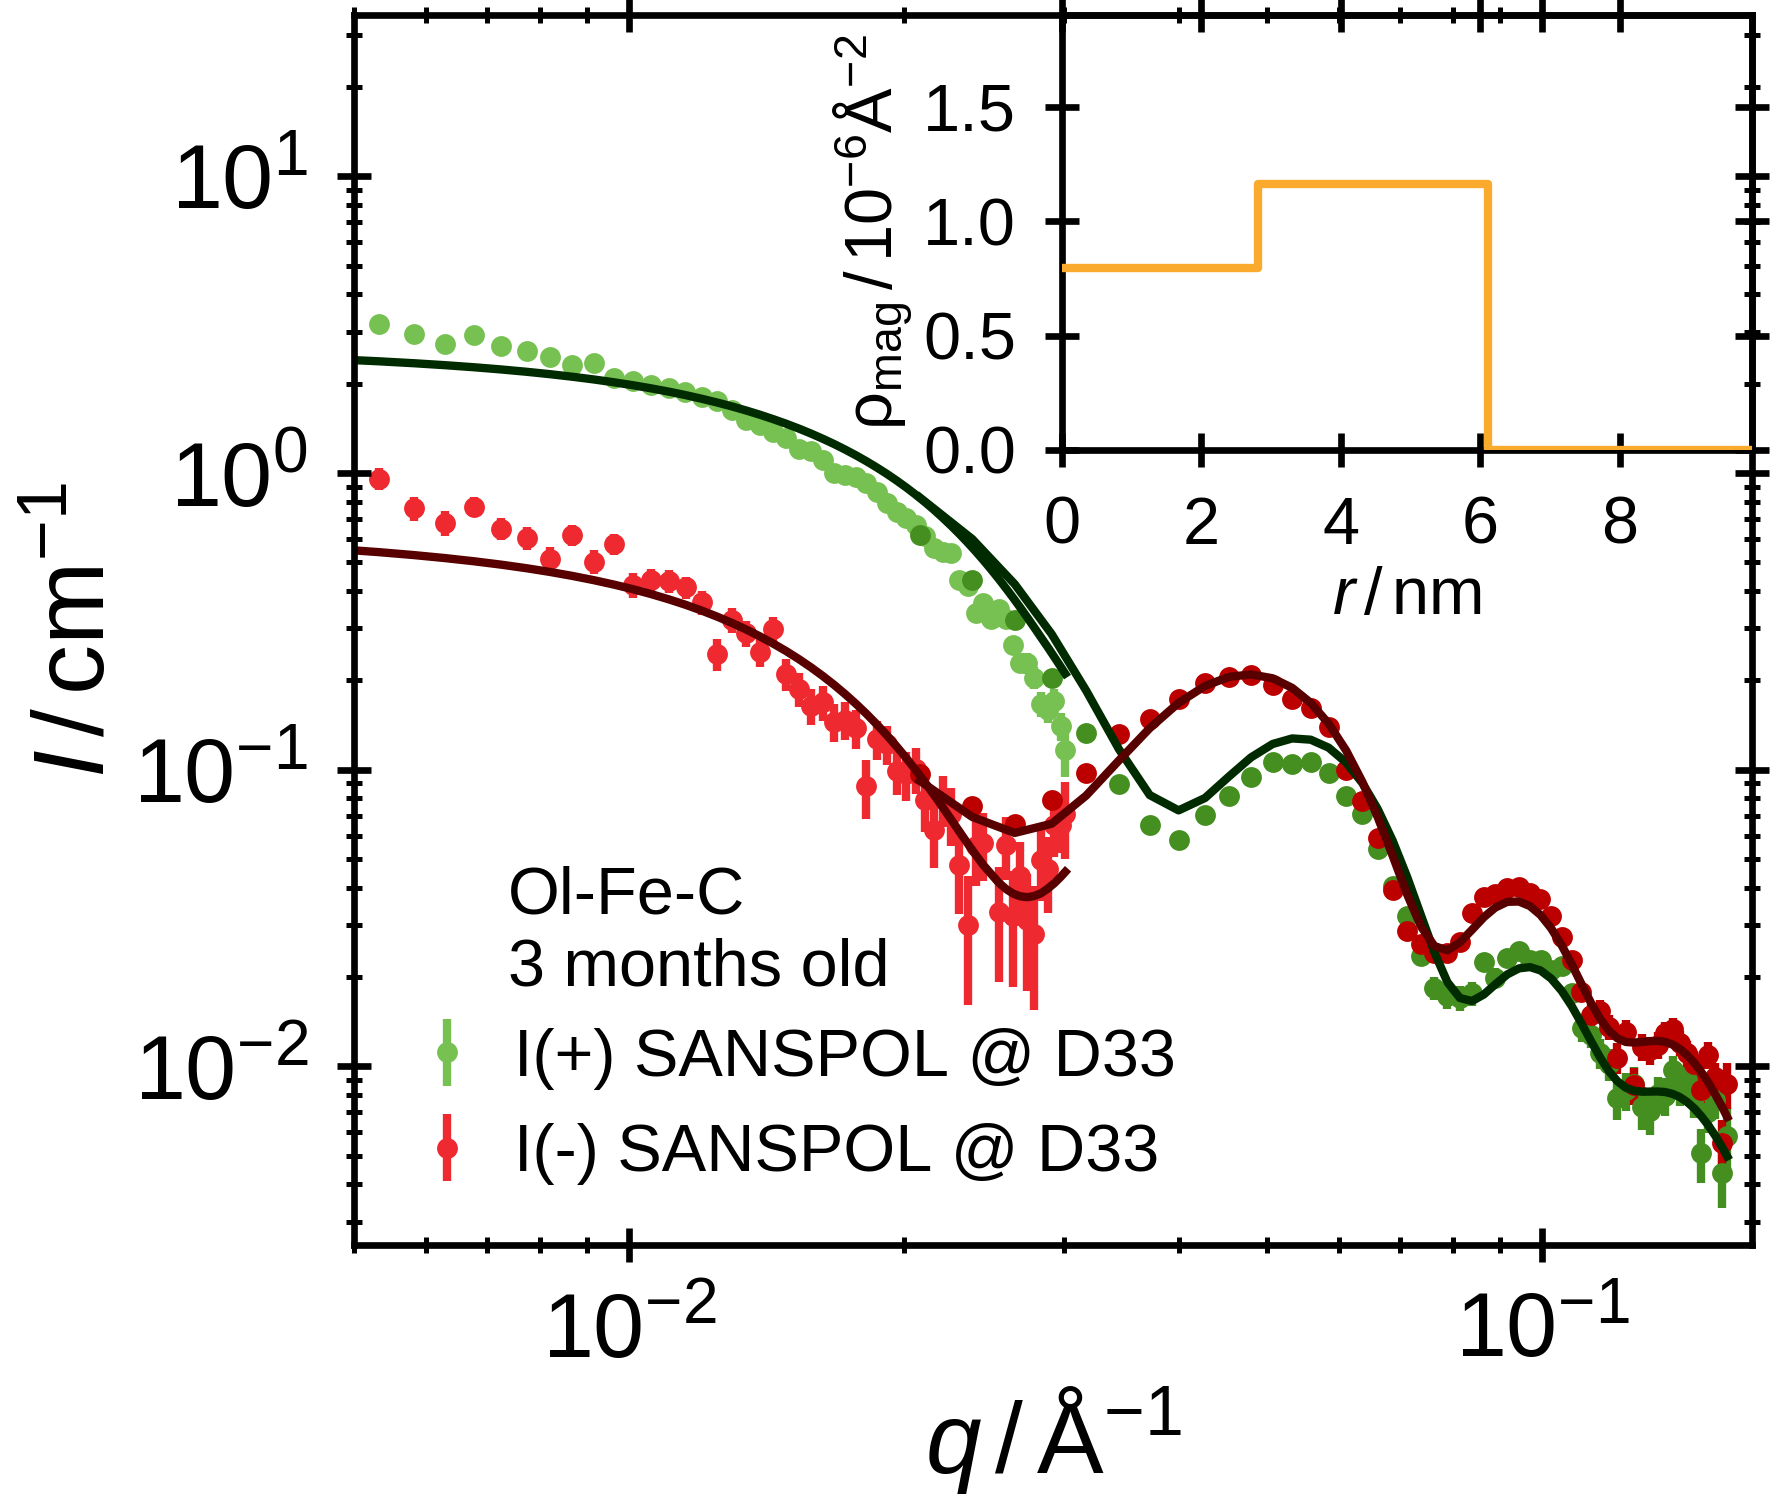
\includegraphics{colloidalCrystals_SAS_Ol-Fe-C_SANSPOL}
      \caption{\label{fig:colloidalCrystals:nanoparticle:sanspol}SANSPOL of Ol-Fe-C with a fit of the magnetic superball form factor.}
    \end{figure}

    To determine the magnetic form factor, the marked $20 ^\circ$ sector is azimuthally integrated and shown in \reffig{fig:colloidalCrystals:nanoparticle:sanspol}.
    Using the same structural parameters for the magnetic form factor, the magnetic scattering length density of the core and shell are refined with the best results shown as solid line in the figure, and the profile of the magnetic form factor along a principal axis of the superball in the inset.
    The magnetic SLD of the core corresponds to a magnetization of $274(64) \unit{kA \, m^{-1}}$ and the SLD of the shell to $399(13) \unit{kA \, m^{-1}}$.
    It is expected that the shell exhibits a stronger magnetization due to it's inverse spinell phase, whereas the core should be only weakly magnetic due to the w\"ustite phase.
    The volume weighted average of the magnetization of the nanocubes is given by $387(13) \unit{kA \, m^{-1}}$.
    This is a lower value than which would be expected from bulk magnetite ($M_\mathrm{magnetite} \eq 475 - 517 \unit{kA \, m^{-1}}$ \cite{Cornell_2003_Their, Handley_2000_Moder}).
    Also the shell is significantly stronger magnetized than what would be expected from a w\"ustite phase, which has at room temperature a paramagnetic susceptibility of $\mu_0 \chi \eq 7230 \cdot 10^{-6}$ \cite{Lide_2004_Handb} and therefore would account for a magnetization of $7.1 \unit{kA \, m^{-1}}$ at $1.234 \unit{T}$.


    \begin{table}[!htbp]
      \centering
      \caption{\label{tab:colloidalCrystals:nanoparticle:sanspol}Parameters for the spherical core-shell model of IOS-11 and IOS-7.}
      \begin{tabular}{ c | l }
        \rule{0pt}{2ex} \textbf{SANSPOL}  & \textbf{Ol-Fe-C} \\
        \hline
        \rule{0pt}{2ex} $\rho^\mathrm{mag}_\mathrm{core} \, / \unit{10^{-6} \angstrom^{-2}}$  & $0.8(2)$ \\
        \rule{0pt}{2ex} $\rho^\mathrm{mag}_\mathrm{shell} \, / \unit{10^{-6} \angstrom^{-2}}$ & $1.11(4)$ \\
        \hline
        \rule{0pt}{2ex} $M_\mathrm{core} \, / \unit{kA m^{-1}}$       & $275(68)$ \\
        \rule{0pt}{2ex} $M_\mathrm{shell} \, / \unit{kA m^{-1}}$      & $382(13)$ \\
        \hline
        \rule{0pt}{2ex} $\bar{M}_\mathrm{particle} \, / \unit{kA m^{-1}}$ & $371(13)$ \\
        \hline
      \end{tabular}
    \end{table}
\end{document}